\chapter{实验结果与分析}

\section{实验设置}

\subsection{实验环境}

本文所有实验均在同一硬件平台上完成，具体配置如表\ref{tab:hardware}所示。

\begin{table}[htbp]
  \centering
  \tablecaption{实验硬件与软件环境配置}
  \label{tab:hardware}
  \resizebox{\textwidth}{!}{%
  \begin{tabular}{lll}
    \hline
    \textbf{类别} & \textbf{配置项} & \textbf{具体参数} \\
    \hline
    \multirow{3}{*}{硬件环境} & 处理器（CPU） & Intel Core i9-14900HX \\
                               & 图形处理器（GPU） & NVIDIA GeForce RTX 4060 Laptop（8GB显存） \\
                               & 内存（RAM） & 32GB DDR5 \\
    \hline
    \multirow{3}{*}{软件环境} & 操作系统 & Windows 11 专业版 \\
                               & CUDA版本 & CUDA 11.8 \\
                               & 深度学习框架 & PyTorch 2.5.1 \\
    \hline
  \end{tabular}%
  }
\end{table}



\subsection{数据集}

为全面评估所提方法在不同水下场景条件下的性能，本文采用两类数据集进行实验，分别覆盖动态水下场景与静态水下场景。

\textbf{（1）动态水下场景数据集}

动态水下场景实验采用UDR-GS\upcite{udrgs2024symmetry}所提供的四个数据子集，每个子集均包含若干连续帧的水下视频图像，具体包括：

\begin{itemize}
  \item \textbf{Robot}：水下机械臂操作场景，共34帧，分辨率为$800\times600$像素。机械臂的往复运动引入了规律性的刚体动态，是测试动态建模精度的典型场景。
  \item \textbf{Fish}：水下鱼类游动场景，记录了多条鱼在珊瑚礁附近自由游动的过程。鱼体的非刚性快速运动对动态建模提出了较高要求。
  \item \textbf{Coral}：珊瑚礁随水流摆动场景，呈现出软体珊瑚枝条在水流驱动下的周期性缓慢摆动，是典型的连续形变动态场景。
  \item \textbf{Streaks}：水下光线焦散或光纹场景，由水面折射形成的动态光纹投影于水底，光斑形状随时间不断变化，对场景外观建模构成挑战。
\end{itemize}

图\ref{fig:dynamic_dataset_samples}展示了四个动态水下场景数据集的示例图像。

\begin{figure}[htbp]
  \centering
  \setlength{\tabcolsep}{2pt}
  \begin{tabular}{cccc}
    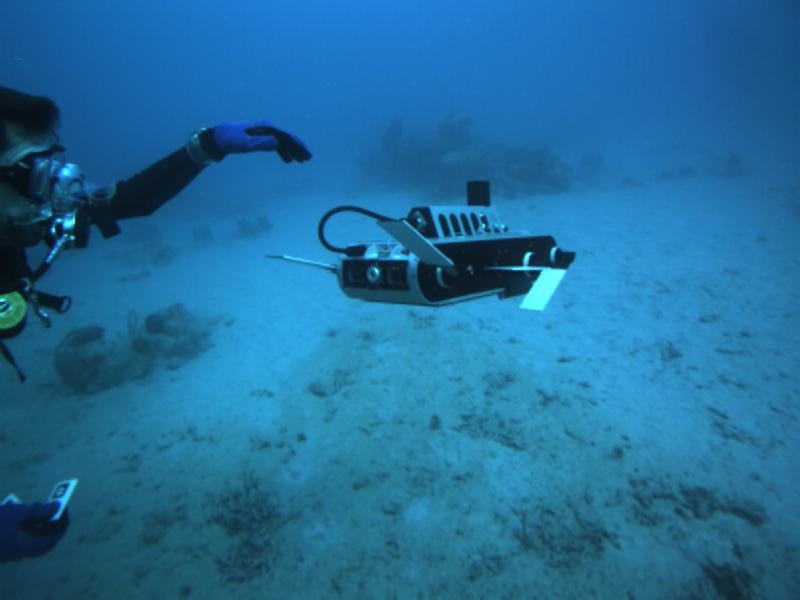
\includegraphics[width=0.23\textwidth]{figures/dataset_samples/robot_sample.jpg} &
    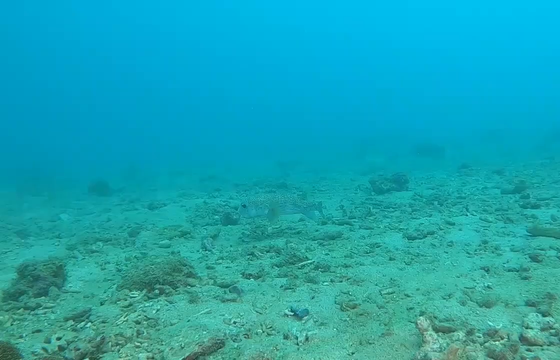
\includegraphics[width=0.23\textwidth]{figures/dataset_samples/fish_sample.png} &
    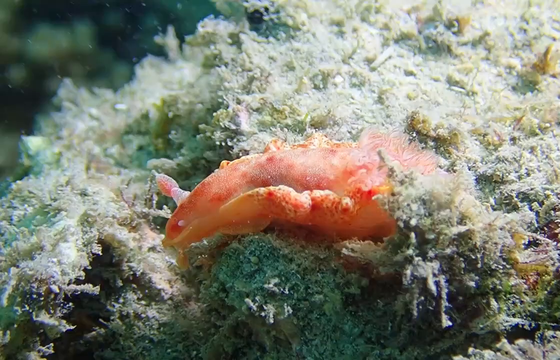
\includegraphics[width=0.23\textwidth]{figures/dataset_samples/coral_sample.png} &
    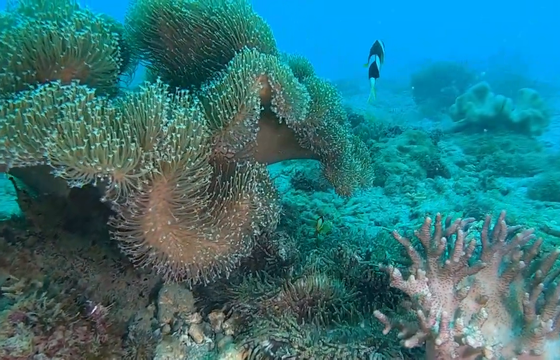
\includegraphics[width=0.23\textwidth]{figures/dataset_samples/streaks_sample.png} \\
    (a) Robot & (b) Fish & (c) Coral & (d) Streaks \\
  \end{tabular}
  \caption{动态水下场景数据集示例图像。(a) Robot：水下机械臂操作场景；(b) Fish：鱼类游动场景；(c) Coral：珊瑚摆动场景；(d) Streaks：水下光纹场景。}
  \label{fig:dynamic_dataset_samples}
\end{figure}

\textbf{（2）静态水下场景数据集}

静态水下场景实验采用SeaThru-NeRF数据集，包含四个典型水下拍摄地点：

\begin{itemize}
  \item \textbf{Curasao}：加勒比海库拉索岛近岸礁盘场景，水体清澈，色偏程度中等。
  \item \textbf{IUI3-RedSea}：红海水下研究站附近场景，水体可见度较高，场景包含丰富的珊瑚与礁石结构。
  \item \textbf{JapaneseGardens-RedSea}：红海Japanese Gardens珊瑚礁场景，细粒度纹理丰富，适合检验方法在复杂静态结构下的外观建模能力。
  \item \textbf{Panama}：巴拿马热带海域场景，水体略浑浊，散射效应相对明显。
\end{itemize}

图\ref{fig:static_dataset_samples}展示了SeaThru-NeRF数据集中四个静态水下场景的示例图像。

\begin{figure}[htbp]
  \centering
  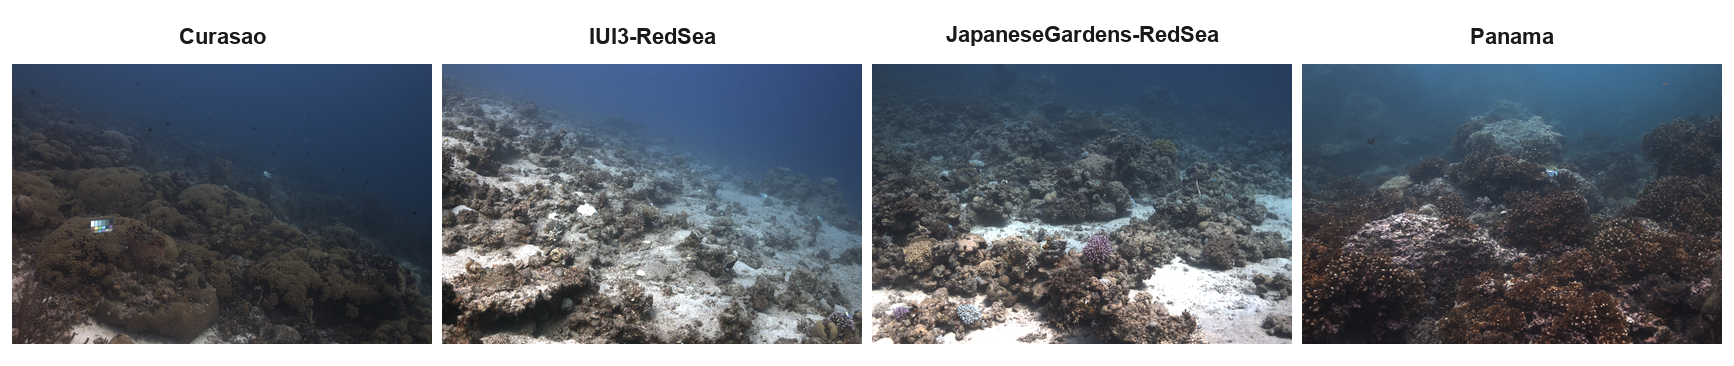
\includegraphics[width=\textwidth]{figures/dataset_samples/static_seathru_samples.png}
  \caption{SeaThru-NeRF静态水下场景数据集示例图像。四个子图依次对应Curasao、IUI3-RedSea、JapaneseGardens-RedSea与Panama场景。}
  \label{fig:static_dataset_samples}
\end{figure}

上述数据集的组合能够有效检验所提方法在处理动态运动、水下色偏与散射等多种挑战时的综合性能。

\subsection{评估指标}

本文采用以下三项广泛使用的图像质量评估指标对各方法进行定量评价。

\textbf{（1）峰值信噪比（PSNR）}

峰值信噪比（Peak Signal-to-Noise Ratio，PSNR）是衡量像素级重建精度的经典指标，其定义为：

\begin{equation}
  \mathrm{PSNR} = 10 \cdot \log_{10} \left( \frac{L^2}{\mathrm{MSE}} \right).
  \label{eq:psnr}
\end{equation}
其中，$L$为像素最大值；若图像归一化至$[0,1]$，则$L=1$，若在8位像素空间计算，则$L=255$；$\mathrm{MSE}$为均方误差。PSNR以分贝（dB）为单位，数值越高表示渲染图像与真实图像在像素层面的偏差越小，重建精度越高。

\textbf{（2）结构相似性指数（SSIM）}

结构相似性指数（Structural Similarity Index，SSIM）\upcite{wang2004ssim}从亮度、对比度与结构三个维度综合衡量图像质量，比PSNR更接近人类视觉感知特性，取值范围为$[0,1]$，数值越接近1表示感知质量越好。

\textbf{（3）感知图像块相似度（LPIPS）}

感知图像块相似度（Learned Perceptual Image Patch Similarity，LPIPS）\upcite{zhang2018lpips}利用预训练深度神经网络提取的高层语义特征计算图像间的感知距离。与PSNR和SSIM不同，LPIPS数值越低表示渲染结果与参考图像在感知质量上越接近，更能反映人类对图像细节与纹理质量的主观判断。

\subsection{对比方法}

为全面评估所提方法的性能，本文选取以下四种具有代表性的基线方法进行对比：

\begin{itemize}
  \item \textbf{3DGS}：原始三维高斯溅射方法\upcite{kerbl2023gaussian}，不包含水下物理模型，也不具备动态场景建模能力，作为基础基线。
  \item \textbf{4DGS}：四维高斯溅射方法\upcite{wu2024gaussian}，通过引入时间维度扩展实现动态场景建模，但不包含水下物理退化模型，代表动态重建的主流基线。
  \item \textbf{SeaSplat}：静态水下高斯溅射方法\upcite{seasplat2025icra}，将水下物理成像模型集成至3DGS框架，能够处理色偏与散射问题，但仅针对静态场景设计，代表静态水下重建基线。
  \item \textbf{UDR-GS}：基于深度正则化的动态水下高斯溅射方法\upcite{udrgs2024symmetry}，同时具备动态建模与水下图像处理能力。
\end{itemize}



\section{动态场景实验结果}

\subsection{定量实验分析}

表\ref{tab:psnr_dynamic}给出了各方法在四个动态水下场景上的PSNR（单位：dB）定量对比结果。每列最优值以\textbf{粗体}标注。

\begin{table}[htbp]
  \centering
  \tablecaption{各方法在动态水下场景上的PSNR对比（单位：dB，越高越好）}
  \label{tab:psnr_dynamic}
  \begin{tabular}{lccccc}
    \hline
    \textbf{方法} & \textbf{Robot} & \textbf{Fish} & \textbf{Coral} & \textbf{Streaks} & \textbf{平均值} \\
    \hline
    3DGS\upcite{kerbl2023gaussian}       & 28.59 & 24.66 & 26.78 & 26.47 & 26.63 \\
    4DGS\upcite{wu2024gaussian}          & 29.49 & 29.09 & 31.14 & 28.81 & 29.63 \\
    UDR-GS\upcite{udrgs2024symmetry}     & 29.62 & \textbf{29.24} & 32.43 & 28.91 & 30.05 \\
    SeaSplat\upcite{seasplat2025icra}    & 28.21 & 23.30 & 26.58 & 26.16 & 26.06 \\
    \textbf{本文方法}                    & \textbf{29.71} & 28.52 & \textbf{33.29} & \textbf{30.65} & \textbf{30.54} \\
    \hline
  \end{tabular}
\end{table}

由表\ref{tab:psnr_dynamic}可以得出以下结论：

\textbf{第一}，本文方法在四个动态场景中的三个（Robot、Coral、Streaks）均取得最优PSNR，平均PSNR为30.54 dB，相较于最接近的基线UDR-GS（30.05 dB）提升约1.6\%，相较于4DGS（29.63 dB）提升约3.1\%，展现出所提方法在动态水下场景上的综合优势。

\textbf{第二}，在Fish场景中，本文方法（28.52 dB）略低于UDR-GS（29.24 dB），差距约为2.5\%。分析认为，Fish场景中鱼体运动速度快且无规律性，快速运动区域的颜色信息在多帧间变化剧烈，水下颜色恢复模块在此类场景中与动态建模模块存在一定程度的梯度干扰，导致两者联合优化时出现轻微的性能损失。UDR-GS专注于几何一致性建模，不引入颜色恢复的额外约束，因此在该场景上表现更为稳定。

\textbf{第三}，两种静态方法（3DGS与SeaSplat）在所有动态场景上均明显落后于动态方法，证明动态建模能力对于处理含运动元素的水下场景至关重要。

\textbf{多指标综合对比。}为进一步评估各方法的感知质量，表\ref{tab:multi_metric}给出了本文方法与基线UDR-GS在四个动态场景上的PSNR、SSIM与LPIPS三项指标的综合对比。

\begin{table}[htbp]
  \centering
  \tablecaption{本文方法与UDR-GS在动态场景上的多指标综合对比}
  \label{tab:multi_metric}
  \begin{tabular}{lcccccc}
    \hline
    \multirow{2}{*}{\textbf{场景}} & \multicolumn{3}{c}{\textbf{本文方法}} & \multicolumn{3}{c}{\textbf{UDR-GS\upcite{udrgs2024symmetry}}} \\
    \cline{2-7}
    & PSNR$\uparrow$ & SSIM$\uparrow$ & LPIPS$\downarrow$ & PSNR$\uparrow$ & SSIM$\uparrow$ & LPIPS$\downarrow$ \\
    \hline
    Robot   & \textbf{29.71} & \textbf{0.9387} & 0.1587          & 29.62 & 0.9312 & \textbf{0.0840} \\
    Fish    & 28.52          & 0.8218          & \textbf{0.1374} & \textbf{29.24} & \textbf{0.8231} & 0.1514 \\
    Coral   & \textbf{33.29} & \textbf{0.9640} & 0.0493          & 32.43 & 0.9475 & \textbf{0.0479} \\
    Streaks & \textbf{30.65} & \textbf{0.9349} & \textbf{0.0605} & 28.91 & 0.8648 & 0.0883 \\
    \hline
  \end{tabular}
\end{table}

综合三项指标可以观察到：在Robot与Coral场景中，本文方法在PSNR和SSIM上均优于UDR-GS，但LPIPS略高；在Streaks场景中，本文方法在全部三项指标上均明显优于UDR-GS，PSNR提升1.74 dB（+6.0\%），SSIM提升0.0701（+8.1\%），LPIPS降低0.0278（$-$31.5\%），提升幅度最为显著；在Fish场景中，本文方法LPIPS更低（0.1374 vs 0.1514），即感知质量更优，但PSNR与SSIM略逊。

\section{静态水下场景实验结果}

为进一步评估本文方法在静态水下场景上的迁移能力，本文在SeaThru-NeRF\upcite{levy2023seathrunerf}数据集所提供的四个典型水下场景上进行实验，包括Curaçao、IUI3-RedSea、JapaneseGardens-RedSea与Panama。对比方法包括原始3DGS\upcite{kerbl2023gaussian}、SeaThru-NeRF\upcite{levy2023seathrunerf}（下表中简记为STN）、SeaSplat\upcite{seasplat2025icra}以及未引入水下物理模型的原始4DGS\upcite{wu2024gaussian}。其中3DGS、4DGS、STN与SeaSplat的指标取自SeaSplat论文公开报告。表\ref{tab:psnr_static}给出了PSNR/SSIM/LPIPS三项指标的综合对比，每行最优值以\textbf{粗体}标注。

\begin{table}[htbp]
  \centering
  \tablecaption{静态水下场景（SeaThru-NeRF\upcite{levy2023seathrunerf}数据集）多方法定量对比（PSNR$\uparrow$ / SSIM$\uparrow$ / LPIPS$\downarrow$）}
  \label{tab:psnr_static}
  \resizebox{\textwidth}{!}{%
  \begin{tabular}{lccccc}
    \hline
    \textbf{场景} & \textbf{3DGS}\upcite{kerbl2023gaussian} & \textbf{STN}\upcite{levy2023seathrunerf} & \textbf{SeaSplat}\upcite{seasplat2025icra} & \textbf{4DGS}\upcite{wu2024gaussian} & \textbf{本文方法} \\
    \hline
    Curaçao                & 28.01 / 0.88 / 0.21          & 30.08 / 0.87 / 0.27 & \textbf{30.30 / 0.90 / 0.19} & 28.05 / 0.75 / 0.40 & 28.82 / 0.77 / 0.26 \\
    IUI3-RedSea            & 21.11 / 0.81 / 0.29          & 26.01 / 0.79 / 0.32 & \textbf{26.67 / 0.87 / 0.21} & 24.43 / 0.68 / 0.41 & 25.27 / 0.72 / 0.34 \\
    JapaneseGardens-RedSea & 21.47 / 0.85 / 0.22          & 21.74 / 0.77 / 0.29 & 22.70 / \textbf{0.87 / 0.18} & 21.81 / 0.76 / 0.33 & \textbf{23.38} / 0.81 / 0.24 \\
    Panama                 & \textbf{29.64 / 0.90} / 0.17 & 27.69 / 0.83 / 0.28 & 28.76 / \textbf{0.90 / 0.15} & 25.63 / 0.75 / 0.37 & 26.86 / 0.80 / 0.33 \\
    \hline
  \end{tabular}%
  }
\end{table}

为进一步从视觉层面对静态场景结果进行比较，图\ref{fig:static_multimethod_curacao}至图\ref{fig:static_multimethod_panama}给出了五种方法在四个SeaThru-NeRF场景上的代表性渲染结果及对应深度图。每幅图对应一个数据集，列方向依次为3DGS、SeaThru-NeRF（STN）、SeaSplat、4DGS与本文方法，上行为渲染结果，下行为深度图。由于整理得到的3DGS结果未包含对应深度输出，图中以N/A标记。

\begin{figure}[htbp]
  \centering
  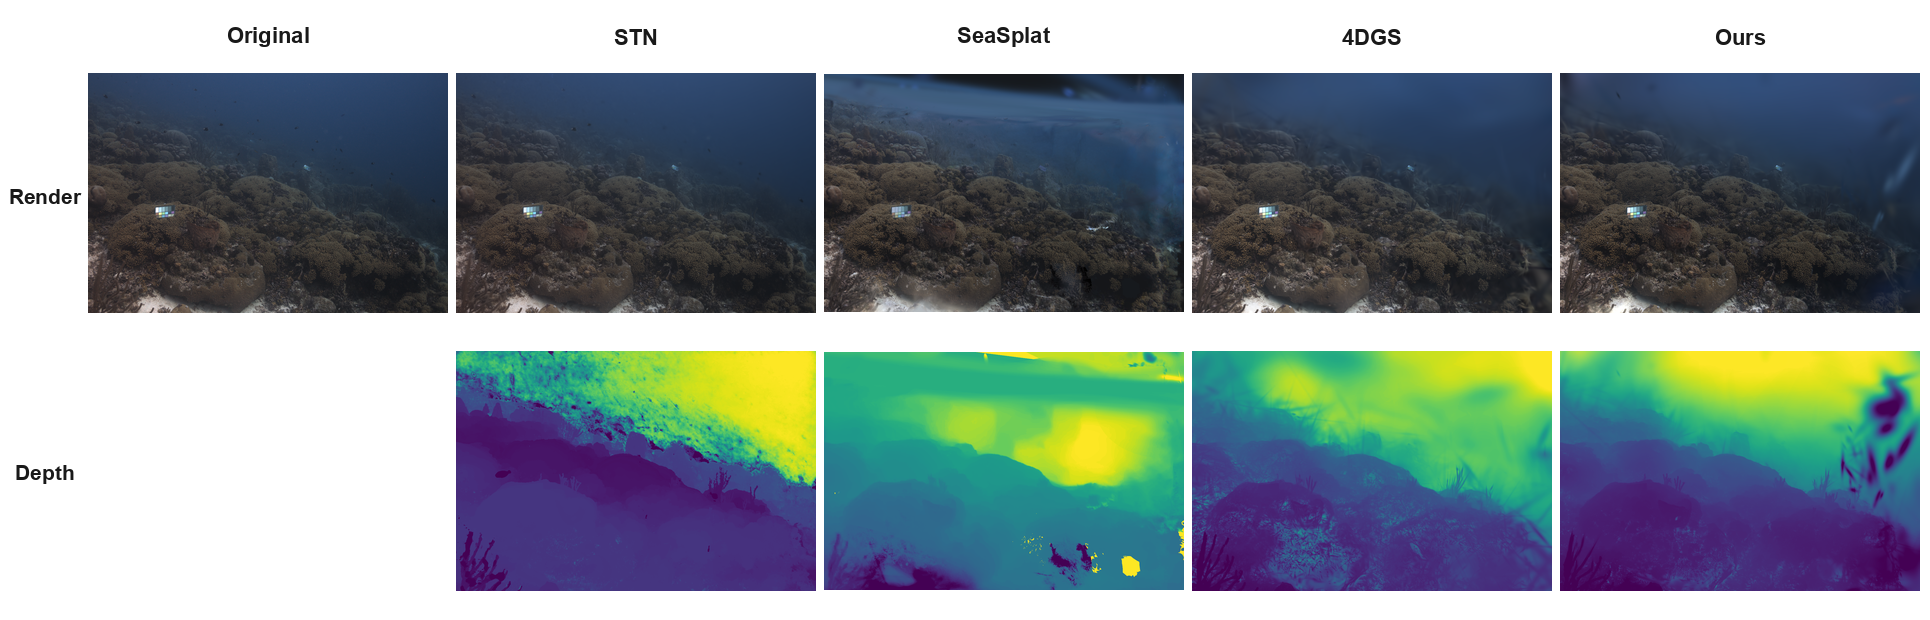
\includegraphics[width=\textwidth]{figures/static_multimethod/curacao_static_models_depth.png}
  \caption{Curaçao场景五种方法渲染结果与深度图对比。}
  \label{fig:static_multimethod_curacao}
\end{figure}

\begin{figure}[htbp]
  \centering
  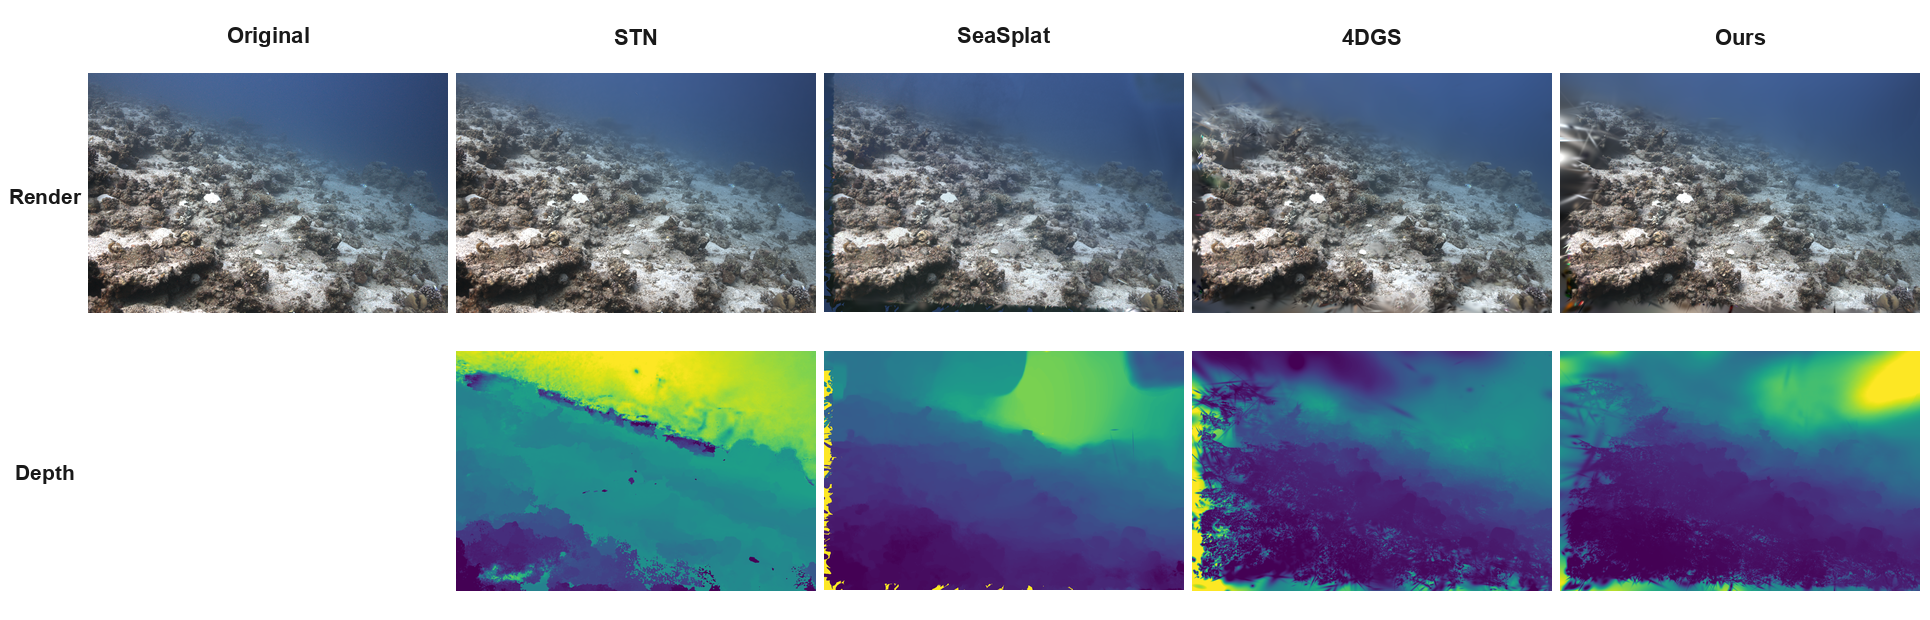
\includegraphics[width=\textwidth]{figures/static_multimethod/iui3_redsea_static_models_depth.png}
  \caption{IUI3-RedSea场景五种方法渲染结果与深度图对比。}
  \label{fig:static_multimethod_iui3}
\end{figure}

\begin{figure}[htbp]
  \centering
  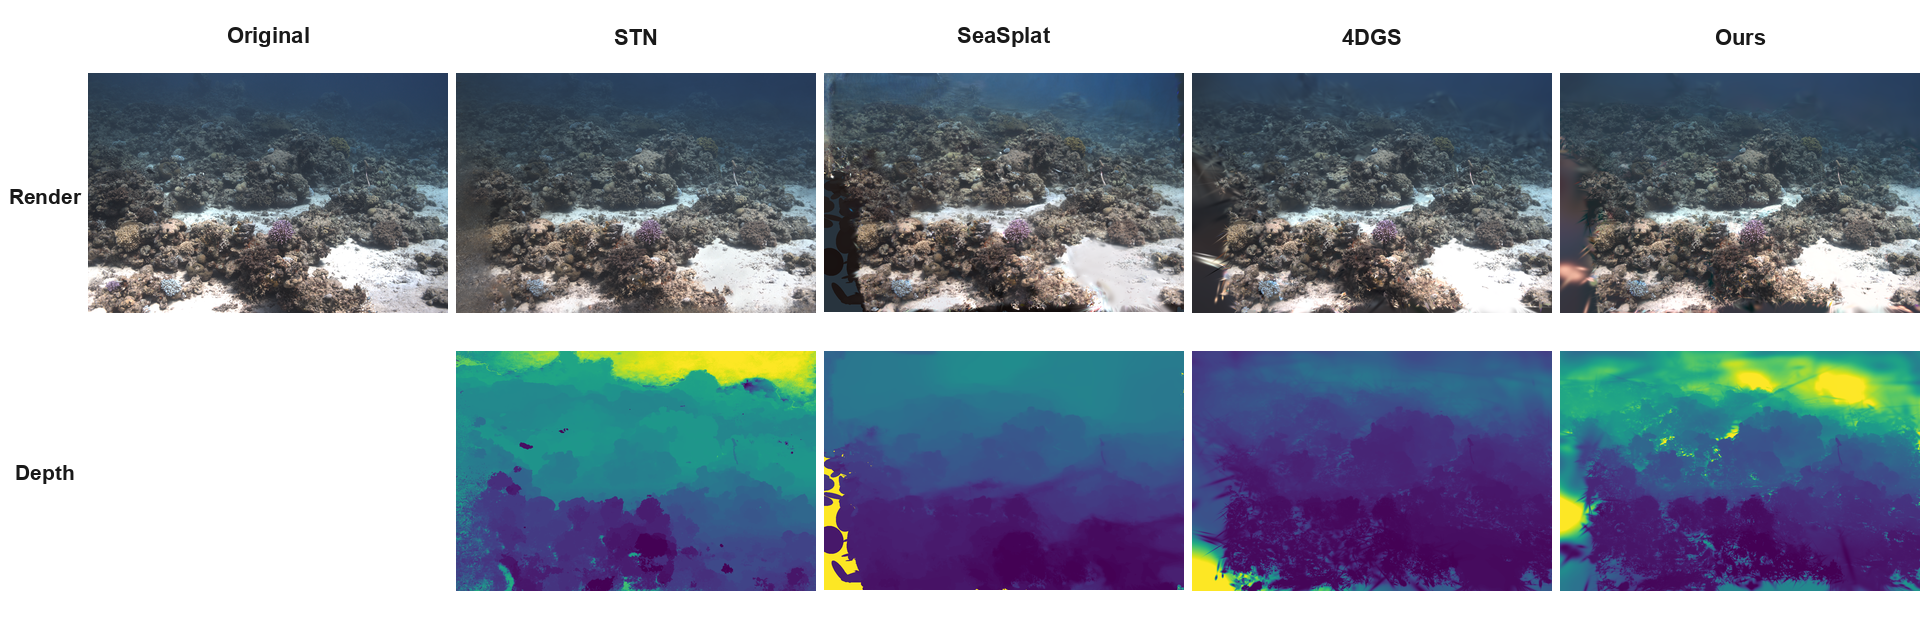
\includegraphics[width=\textwidth]{figures/static_multimethod/japanese_gardens_static_models_depth.png}
  \caption{JapaneseGardens-RedSea场景五种方法渲染结果与深度图对比。}
  \label{fig:static_multimethod_japanese}
\end{figure}

\begin{figure}[htbp]
  \centering
  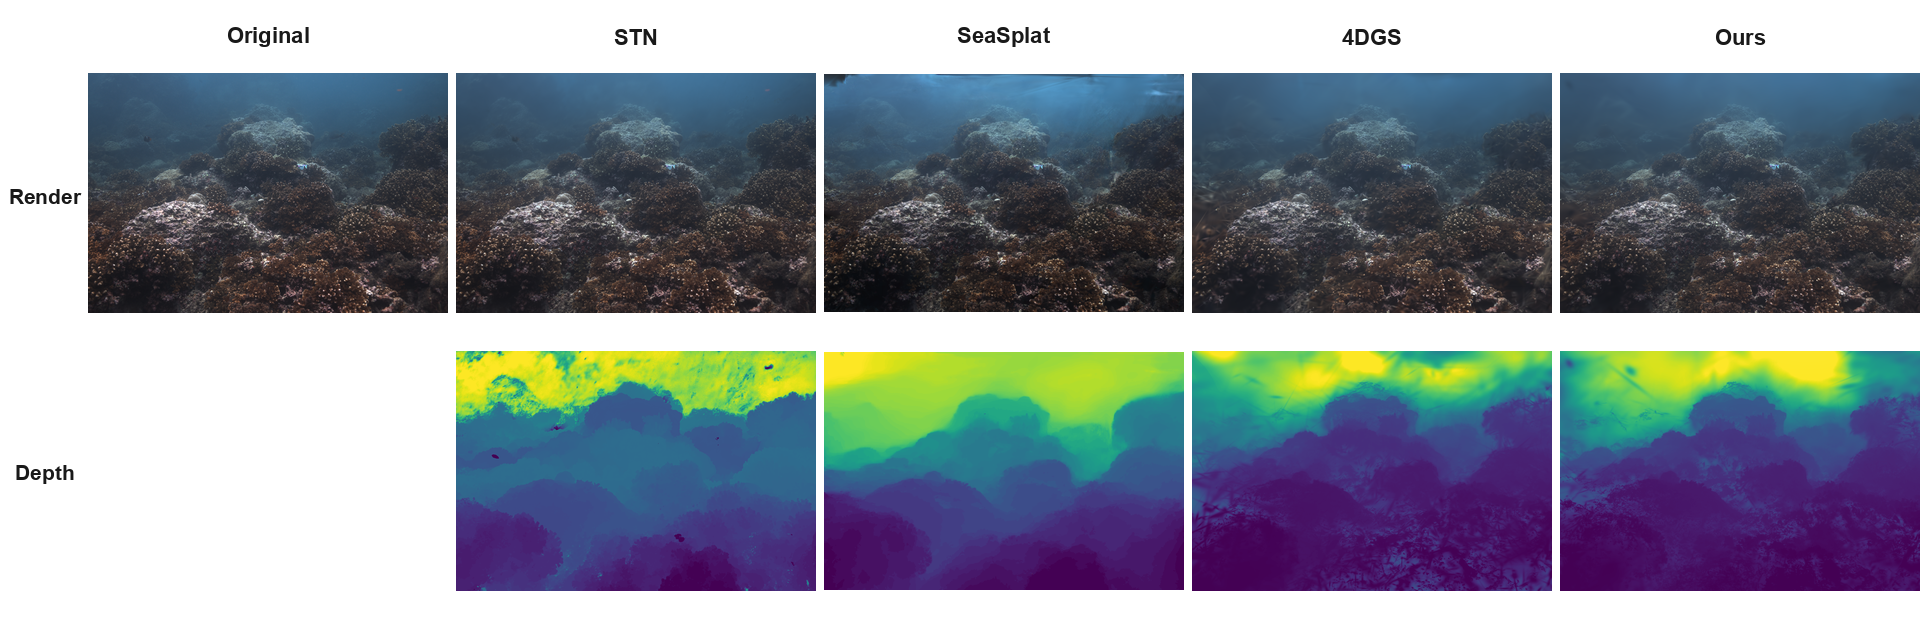
\includegraphics[width=\textwidth]{figures/static_multimethod/panama_static_models_depth.png}
  \caption{Panama场景五种方法渲染结果与深度图对比。}
  \label{fig:static_multimethod_panama}
\end{figure}

\subsection{JapaneseGardens-RedSea渲染与去水结果}

为进一步展示静态复杂珊瑚礁场景中的外观恢复效果，图\ref{fig:static_japanese_dewater}给出了JapaneseGardens-RedSea场景的原图、渲染结果与去水结果。图中列方向依次为原始水下图像、SeaThru-NeRF、SeaSplat与本文方法；行方向分别对应带水渲染结果与依据水下成像模型反演得到的去水结果。

\begin{figure}[htbp]
  \centering
  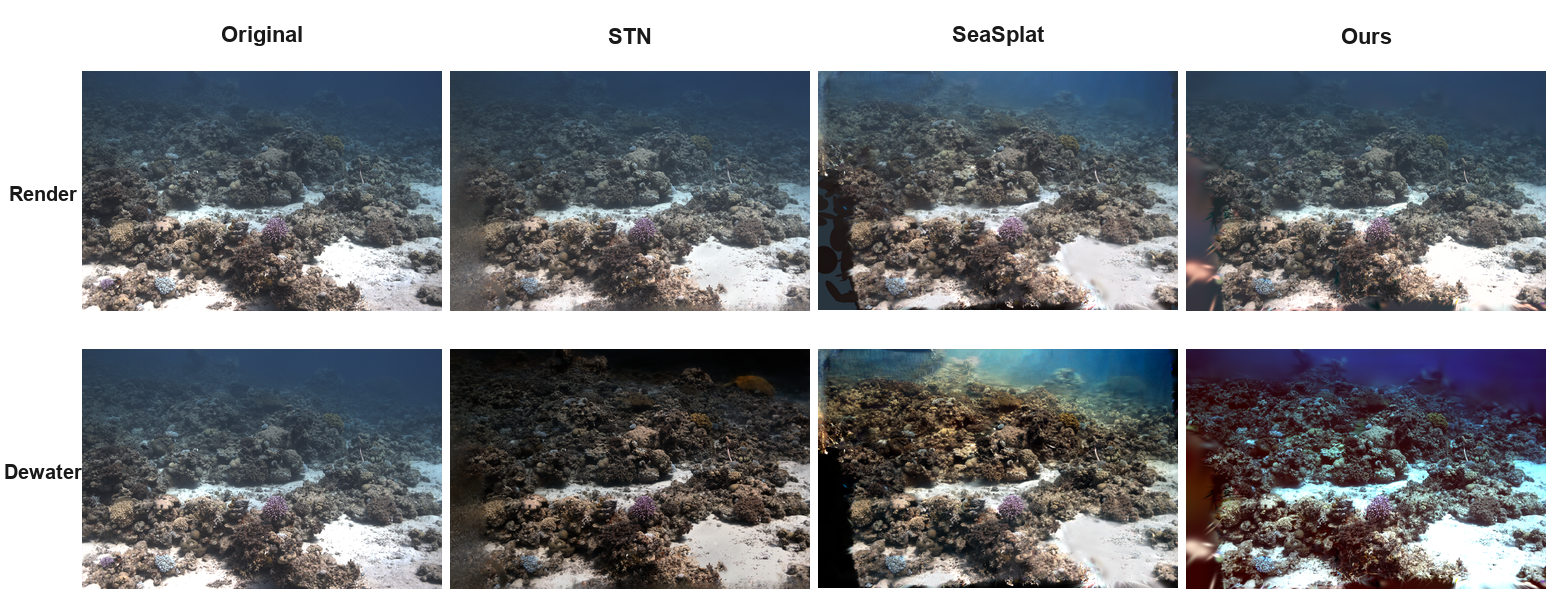
\includegraphics[width=\textwidth]{figures/static_multimethod/japanese_dewater_render_compare.png}
  \caption{JapaneseGardens-RedSea场景原图、渲染结果与去水结果对比。上行为带水渲染结果，下行为去水结果；原图列在两行中重复显示作为参考。}
  \label{fig:static_japanese_dewater}
\end{figure}

由表\ref{tab:psnr_static}可观察到，本文方法在JapaneseGardens-RedSea场景上的PSNR（23.38 dB）超过所有基线，相较SeaSplat提升+0.68 dB，相较4DGS提升+1.57 dB，反映出当场景具有丰富细粒度纹理时，本文方法的水下物理模型与深度监督相结合所带来的联合约束依然能够提供增益；相较于不带水下物理模型的原始4DGS\upcite{wu2024gaussian}，本文方法在所有四个静态场景上的PSNR平均提升约1.05 dB，且SSIM与LPIPS同步改善，表明所引入的水下物理建模能够在动态主干基础上有效补偿静态场景的色偏与散射；本文方法在Curaçao、IUI3-RedSea、Panama上仍略逊于SeaSplat，原因在于SeaSplat专为静态场景优化，而本文方法在这些场景中保留的形变场参数构成不必要的自由度，引入了一定的优化噪声。

此外，本文方法在SaltPond场景上的实验也作为额外的鲁棒性参考。在该场景上，仅使用深度监督而未启用水下优化的配置PSNR为26.11 dB（SSIM为0.6251）；启用完整水下优化后，本文方法PSNR提升至27.15 dB（SSIM为0.7036），相较原始SeaSplat论文报告的27.47 dB仅低0.32 dB。

\section{对比分析}

\subsection{与SeaSplat对比分析}

SeaSplat\upcite{seasplat2025icra}是面向静态场景设计的水下高斯溅射方法，其核心优势在于对水下色偏与散射的物理建模，但由于缺乏动态场景处理能力，其在动态数据集上的性能受到严重制约。

表\ref{tab:psnr_dynamic}中各场景的对比数据清晰地反映了这一局限。在Robot场景中，本文方法PSNR为29.71 dB，而SeaSplat仅为28.21 dB，提升约5.3\%；在Fish场景中，差距最为悬殊，本文方法（28.52 dB）相较于SeaSplat（23.30 dB）提升约22.4\%；在Coral场景中，提升幅度高达25.2\%（33.29 vs 26.58 dB）。

上述差距的原因在于，Fish场景中鱼体的快速游动、Coral场景中珊瑚枝条的持续摆动，以及Robot场景中机械臂的往复运动，均会导致多帧图像之间出现显著的非刚性形变。静态方法（包括SeaSplat）在处理此类输入时，无法将运动信息从场景几何中解耦，使得对应运动区域的高斯体在训练过程中接收到来自不同帧的矛盾监督信号，最终收敛至多帧叠加的模糊状态，导致渲染结果在运动区域出现严重的鬼影与模糊。相比之下，本文方法通过时间相关的形变场对运动进行显式建模，有效消除了上述模糊现象。

SeaSplat在Streaks场景（26.16 dB）上的劣势相对于其他两种静态方法（3DGS为26.47 dB）更为明显，这可能与水下光焦散的时变特性同其水下物理模型的静态假设之间的冲突有关，动态光纹被错误地纳入后向散射项建模，导致模型估计出错。

\subsection{与4DGS和UDR-GS对比分析}

\textbf{（1）Robot场景}

在Robot场景中，本文方法（29.71 dB）略优于4DGS（29.49 dB）和UDR-GS（29.62 dB），三者差距在0.3\%至0.7\%之间。机械臂运动具有规律性，三种动态方法均能较好地建模其运动轨迹，因此差距相对有限。本文方法在SSIM上的优势表明其对机械臂边缘的结构细节刻画更为精确，但LPIPS指标（0.1587）高于UDR-GS（0.0840），反映出在感知质量方面存在一定不足，可能与本文方法引入的水下颜色恢复模块改变了局部纹理的高频特征分布有关。

\textbf{（2）Fish场景}

Fish场景是本文方法的相对薄弱场景。鱼体的快速非规律性运动与颜色恢复模块之间存在梯度冲突：在快速运动区域，形变场的估计误差会导致颜色恢复模块接收到不一致的颜色监督信号，进而干扰水体参数的准确估计。UDR-GS（29.24 dB）由于不引入颜色恢复的额外参数，其优化目标更为单一，在此类高速运动场景下反而获得了更稳定的收敛。这一结果表明，如何在快速运动场景中降低多模块间的梯度干扰，是未来工作需要重点改进的方向之一。

\textbf{（3）Coral场景}

Coral场景最充分地体现了本文方法的综合优势。珊瑚礁场景同时具有动态性（珊瑚摆动）和显著的水下色偏（蓝绿色偏移），这正是本文方法所针对的双重挑战。本文方法PSNR（33.29 dB）相较UDR-GS（32.43 dB）提升+2.7\%，相较4DGS（31.14 dB）提升+6.9\%，SSIM也由0.9475提升至0.9640。这一结果印证了完整水下物理模型在恢复珊瑚礁真实色彩方面的重要作用：4DGS缺乏色彩校正，导致颜色失真使PSNR受损；UDR-GS虽具备一定的水下处理能力，但其颜色恢复能力弱于本文方法，因此在涉及色偏的质量指标上略逊。

\textbf{（4）Streaks场景}

Streaks场景展示了本文方法最显著的性能优势。水下光焦散产生的时变光纹不仅是一种动态现象，更与水体的光学散射特性密切相关。本文方法通过动态高斯建模捕捉光纹的时变形态，同时通过水下物理模型将光焦散的颜色特性与环境散射项解耦，两个模块形成协同效应。PSNR提升1.74 dB（从28.91至30.65 dB），SSIM提升8.1\%（从0.8648至0.9349），LPIPS降低31.5\%（从0.0883至0.0605），三项指标全面领先，充分验证了动态建模与水下物理建模联合设计的有效性。



\section{可视化结果}

\subsection{渲染效果对比}

图\ref{fig:render_compare}展示了本文方法与SeaSplat在四个动态场景上的渲染效果对比。每行对应一个动态水下场景（Robot、Coral、Fish、Streaks），每列从左至右依次为：测试视角采集到的原始水下参考图像（GT）、SeaSplat的渲染图像、SeaSplat的深度图（以热力图显示）、本文方法的渲染结果、本文方法的深度图（以热力图显示）。深度图颜色仅表示相对远近关系，不代表RGB渲染颜色。通过对比SeaSplat渲染图像与GT，可以观察到静态方法在动态区域容易出现重影与模糊；本文方法在运动区域的轮廓保持更稳定。

\begin{figure}[htbp]
  \centering
  \setlength{\tabcolsep}{1pt}
  \renewcommand{\arraystretch}{0.6}
  \begin{tabular}{@{}>{\centering\arraybackslash}m{1.2em}@{\hspace{2pt}}*{5}{>{\centering\arraybackslash}m{0.17\textwidth}}@{}}
     & GT（原始） & SeaSplat & SeaSplat深度 & 本文方法 & 本文深度 \\
    \rotatebox{90}{Robot}   & 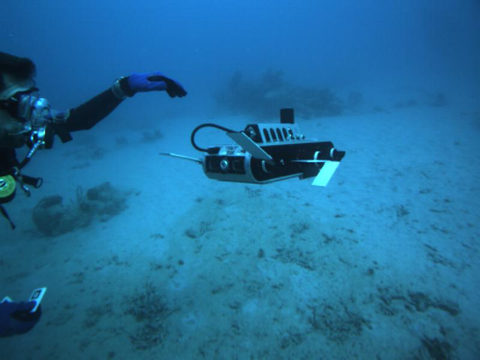
\includegraphics[width=0.17\textwidth]{figures/render_compare/robot_gt.png}   & 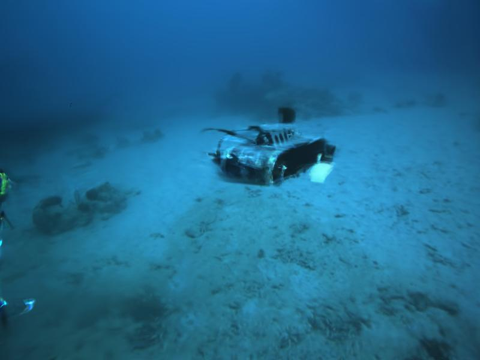
\includegraphics[width=0.17\textwidth]{figures/render_compare/robot_sea_water.png}   & 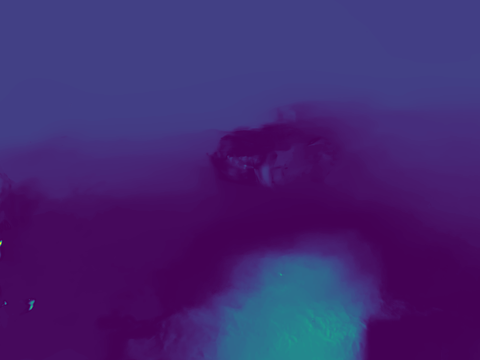
\includegraphics[width=0.17\textwidth]{figures/render_compare/robot_sea_depth.png}   & 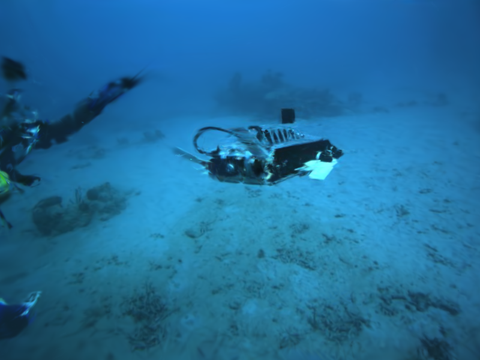
\includegraphics[width=0.17\textwidth]{figures/render_compare/robot_ours.png}   & 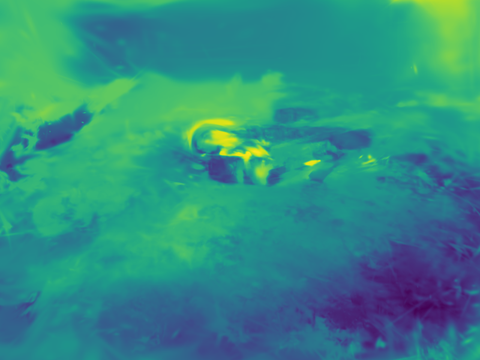
\includegraphics[width=0.17\textwidth]{figures/render_compare/robot_ours_depth.png}   \\
    \rotatebox{90}{Coral}   & 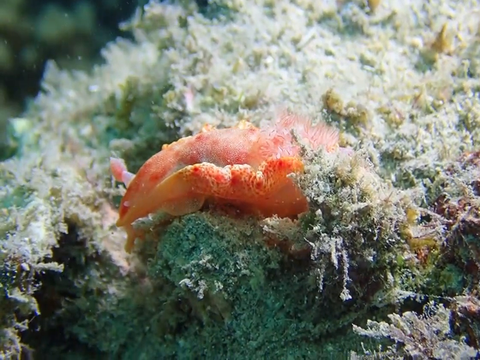
\includegraphics[width=0.17\textwidth]{figures/render_compare/coral_gt.png}   & 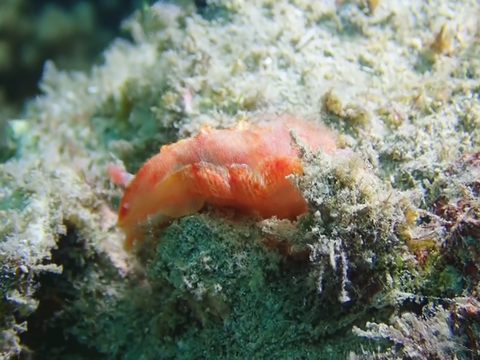
\includegraphics[width=0.17\textwidth]{figures/render_compare/coral_sea_water.png}   & 
\includegraphics[width=0.17\textwidth]{figures/render_compare/coral_sea_depth.png}   & 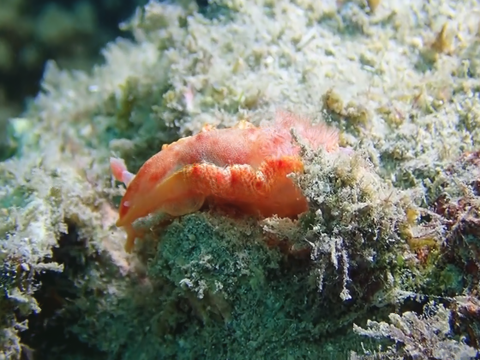
\includegraphics[width=0.17\textwidth]{figures/render_compare/coral_ours.png}   & 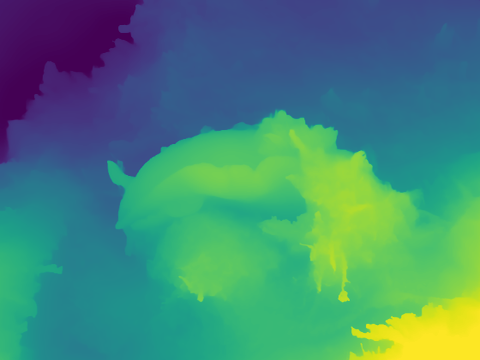
\includegraphics[width=0.17\textwidth]{figures/render_compare/coral_ours_depth.png}   \\
    \rotatebox{90}{Fish}    & 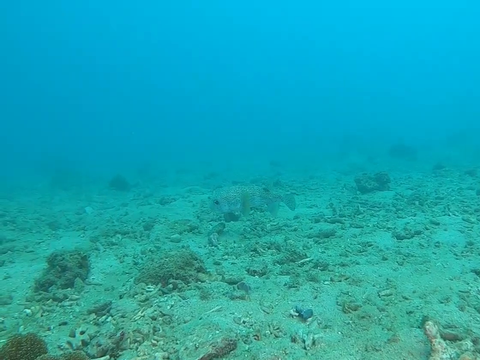
\includegraphics[width=0.17\textwidth]{figures/render_compare/fish_gt.png}    & 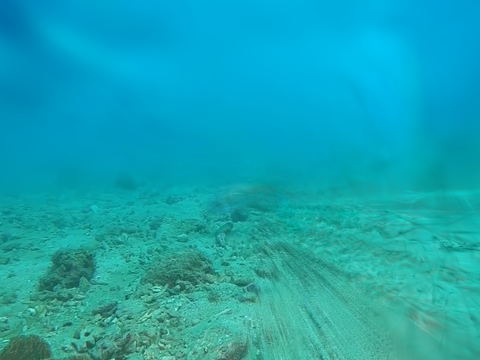
\includegraphics[width=0.17\textwidth]{figures/render_compare/fish_sea_water.png}    & 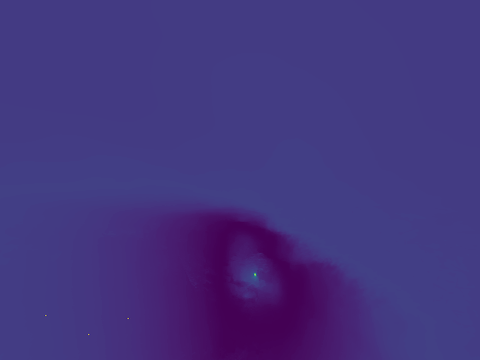
\includegraphics[width=0.17\textwidth]{figures/render_compare/fish_sea_depth.png}    & 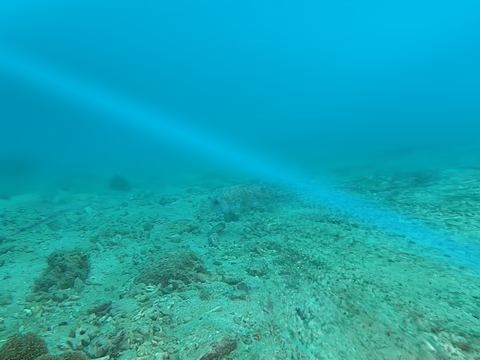
\includegraphics[width=0.17\textwidth]{figures/render_compare/fish_ours.png}    & 
\includegraphics[width=0.17\textwidth]{figures/render_compare/fish_ours_depth.png}    \\
    \rotatebox{90}{Streaks} & \includegraphics[width=0.17\textwidth]{figures/render_compare/streaks_gt.png} & 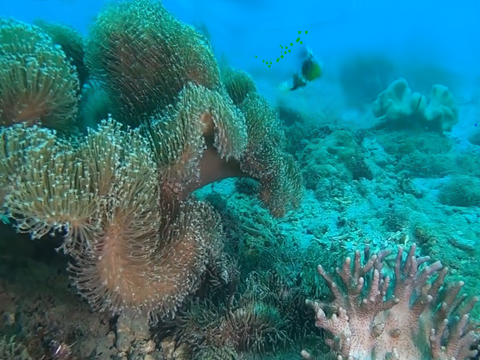
\includegraphics[width=0.17\textwidth]{figures/render_compare/streaks_sea_water.png} & 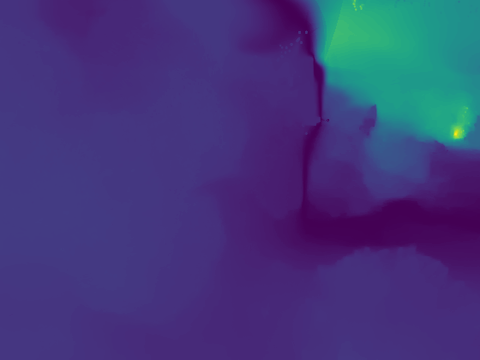
\includegraphics[width=0.17\textwidth]{figures/render_compare/streaks_sea_depth.png} & 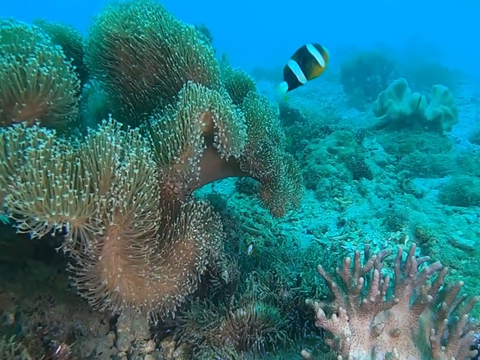
\includegraphics[width=0.17\textwidth]{figures/render_compare/streaks_ours.png} & 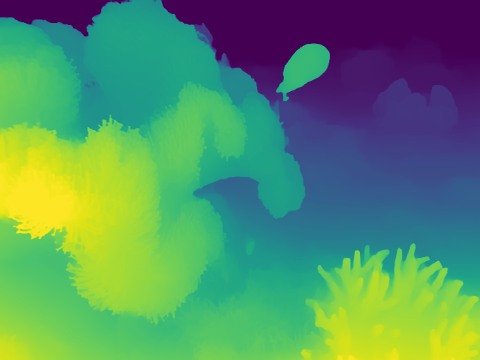
\includegraphics[width=0.17\textwidth]{figures/render_compare/streaks_ours_depth.png} \\
  \end{tabular}
  \caption{四个动态水下场景的渲染效果对比。GT为测试视角采集到的原始水下参考图像；两列深度图为相对深度的热力图显示。与SeaSplat静态基线相比，本文方法在动态区域的重影和轮廓模糊更少。}
  \label{fig:render_compare}
\end{figure}

由图\ref{fig:render_compare}可以观察到，在各个场景中，SeaSplat由于缺乏动态建模能力，在运动物体区域更容易出现重影与模糊；本文方法通过时变高斯形变场显式建模运动，使运动物体轮廓保持相对稳定。需要注意的是，图中深度结果主要用于辅助判断几何连续性，定量结论仍以表\ref{tab:psnr_dynamic}和表\ref{tab:multi_metric}为准。


\subsection{水下去水效果}

图\ref{fig:dewater}展示了本文方法在四个动态水下场景上的水下图像分解效果。每行对应一个场景，其中$\mathbf{I}$表示模型合成的水下观测图像，$\mathbf{J}$表示依据水下成像模型反演得到的干净外观图像，即$\mathbf{J}=(\mathbf{I}-\mathbf{B}(\mathbf{Z}))\oslash\mathbf{A}(\mathbf{Z})$（$\oslash$表示逐元素除法）。这里的"去水"不是额外的图像增强后处理，而是模型内部物理分解得到的外观项。

\begin{figure}[htbp]
  \centering
  \setlength{\tabcolsep}{2pt}
  \renewcommand{\arraystretch}{0.6}
  \begin{tabular}{@{}>{\centering\arraybackslash}m{1.2em}@{\hspace{2pt}}*{5}{>{\centering\arraybackslash}m{0.17\textwidth}}@{}}
     & GT（原始） & SeaSplat $\mathbf{I}$ & SeaSplat $\mathbf{J}$ & 本文 $\mathbf{I}$ & 本文 $\mathbf{J}$ \\
    \rotatebox{90}{Robot}   & 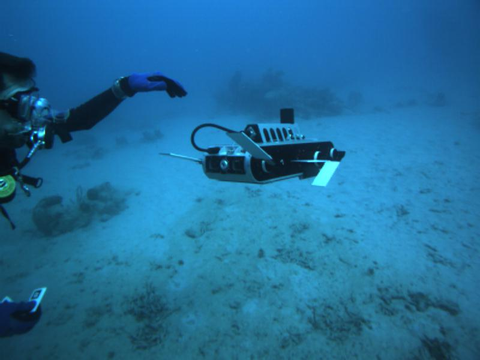
\includegraphics[width=0.17\textwidth]{figures/dewater/robot_gt.png}   & 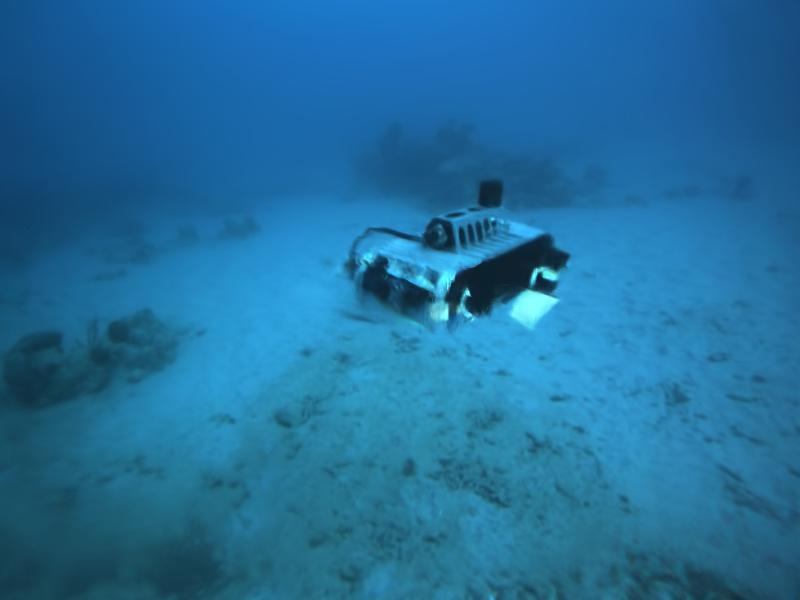
\includegraphics[width=0.17\textwidth]{figures/dewater/robot_sea_I.png}   & 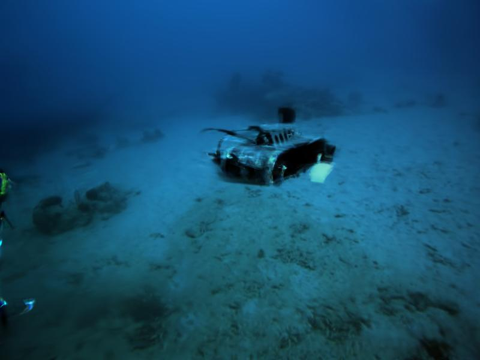
\includegraphics[width=0.17\textwidth]{figures/dewater/robot_sea_J.png}   & 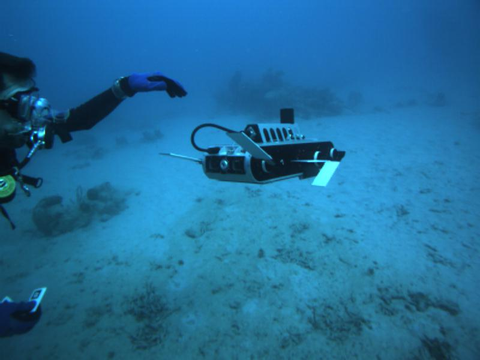
\includegraphics[width=0.17\textwidth]{figures/dewater/robot_ours_I.png}   & 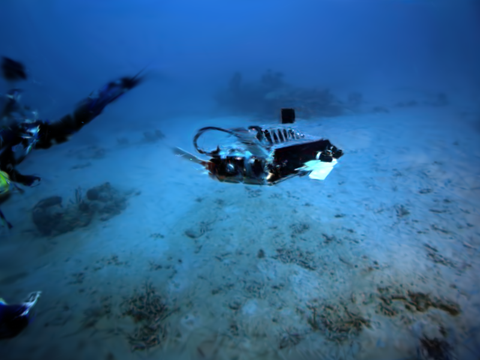
\includegraphics[width=0.17\textwidth]{figures/dewater/robot_ours_J.png}   \\
    \rotatebox{90}{Coral}   & 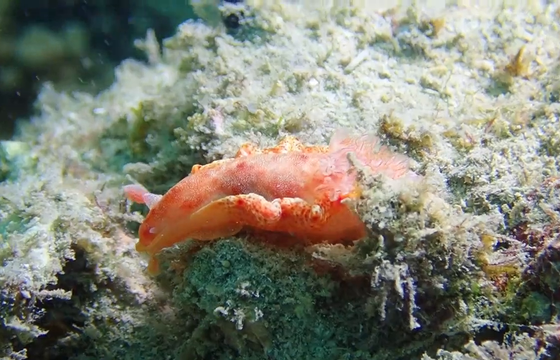
\includegraphics[width=0.17\textwidth]{figures/dewater/coral_gt.png}   & 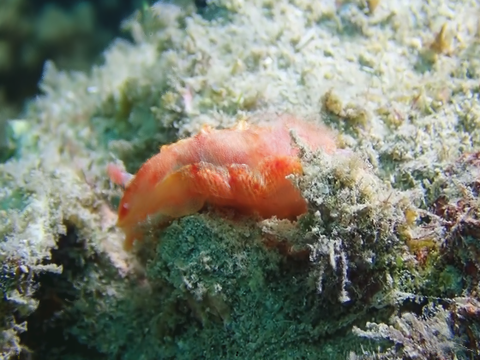
\includegraphics[width=0.17\textwidth]{figures/dewater/coral_sea_I.png}   & 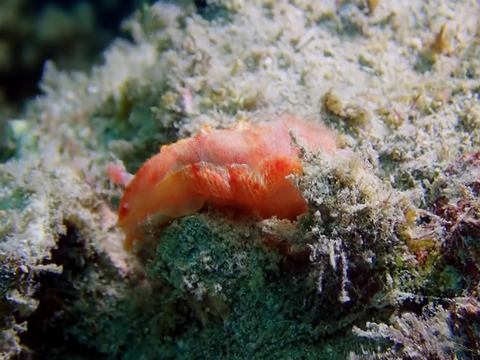
\includegraphics[width=0.17\textwidth]{figures/dewater/coral_sea_J.png}   & 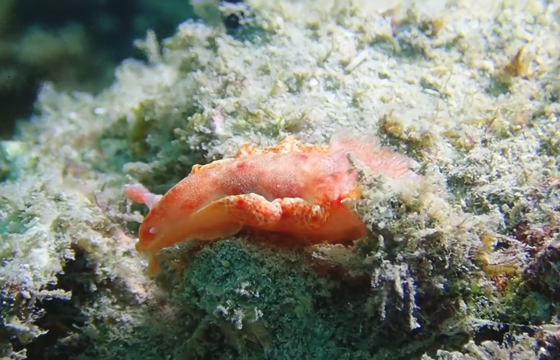
\includegraphics[width=0.17\textwidth]{figures/dewater/coral_ours_I.png}   & 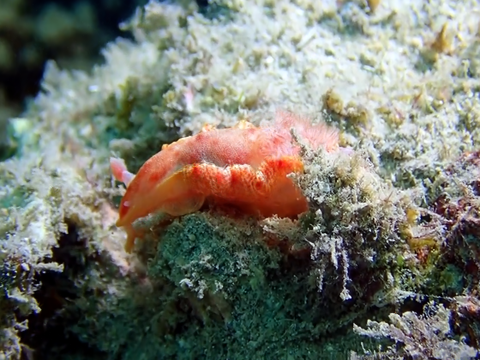
\includegraphics[width=0.17\textwidth]{figures/dewater/coral_ours_J.png}   \\
    \rotatebox{90}{Fish}    & \includegraphics[width=0.17\textwidth]{figures/dewater/fish_gt.png}    & 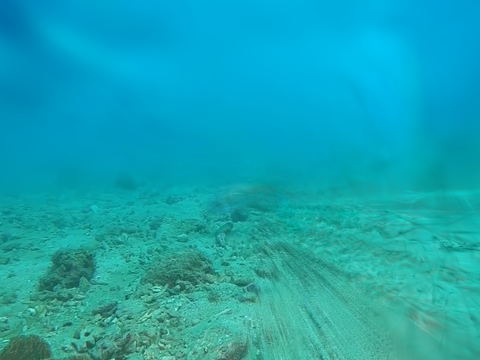
\includegraphics[width=0.17\textwidth]{figures/dewater/fish_sea_I.png}    & 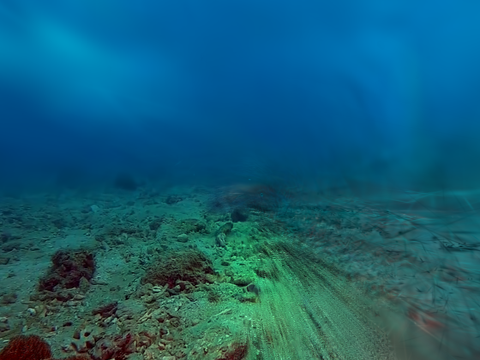
\includegraphics[width=0.17\textwidth]{figures/dewater/fish_sea_J.png}    & 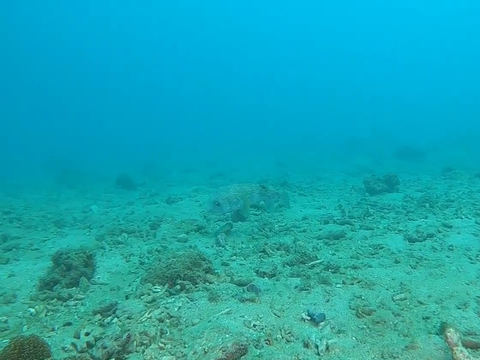
\includegraphics[width=0.17\textwidth]{figures/dewater/fish_ours_I.png}    & 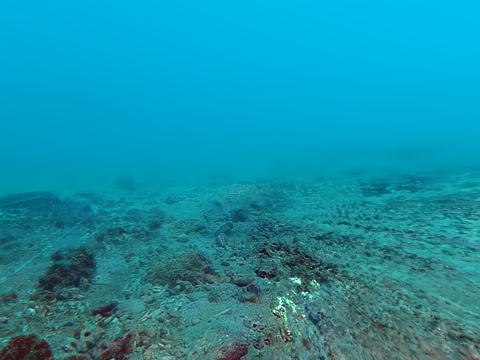
\includegraphics[width=0.17\textwidth]{figures/dewater/fish_ours_J.png}    \\
    \rotatebox{90}{Streaks} & 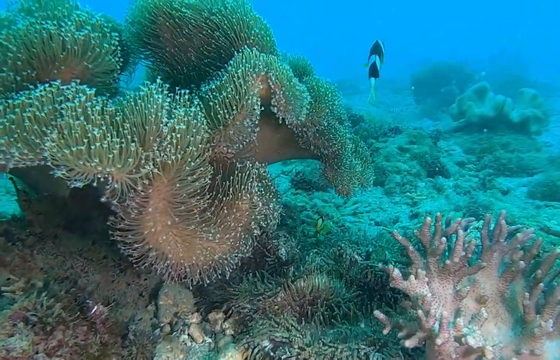
\includegraphics[width=0.17\textwidth]{figures/dewater/streaks_gt.png} & 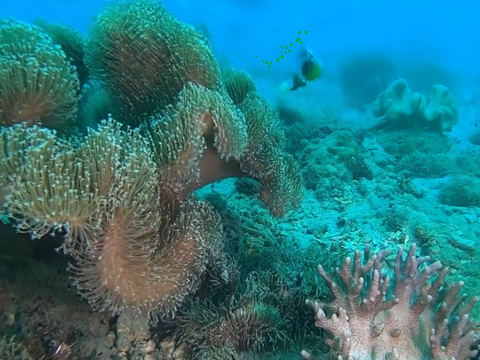
\includegraphics[width=0.17\textwidth]{figures/dewater/streaks_sea_I.png} & 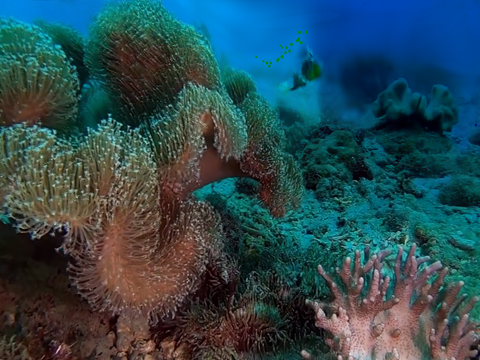
\includegraphics[width=0.17\textwidth]{figures/dewater/streaks_sea_J.png} & 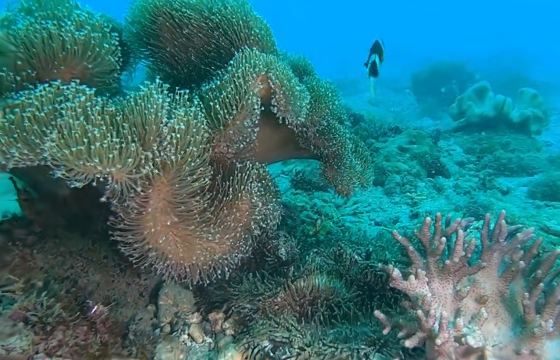
\includegraphics[width=0.17\textwidth]{figures/dewater/streaks_ours_I.png} & 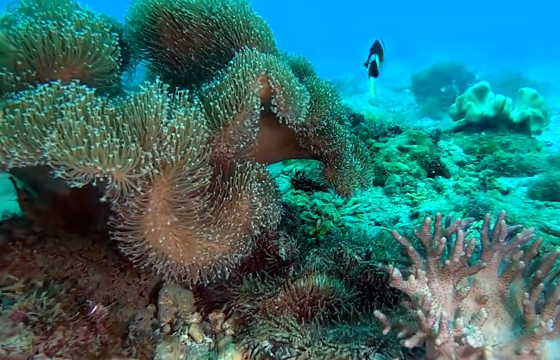
\includegraphics[width=0.17\textwidth]{figures/dewater/streaks_ours_J.png} \\
  \end{tabular}
  \caption{四个动态水下场景的物理分解结果。从左至右依次为：测试视角原始水下参考图像（GT）、SeaSplat渲染水下观测图像$\mathbf{I}$、SeaSplat反演干净外观$\mathbf{J}$、本文方法渲染水下观测图像$\mathbf{I}$、本文方法反演干净外观$\mathbf{J}$。}
  \label{fig:dewater}
\end{figure}

对比图中，本文$\mathbf{I}$与本文$\mathbf{J}$在部分场景下差异并不剧烈，这与两个因素有关：一方面，训练目标直接约束的是与GT一致的水下观测图像$\mathbf{I}$，物理反演项$\mathbf{J}$主要用于约束高斯外观而非追求主观增强效果；另一方面，Robot和Fish等场景的有效可见距离较短，学习到的衰减和后向散射幅度有限，因此反演前后的视觉差异相对温和。该图更适合说明模型是否形成了可解释的$\mathbf{I}/\mathbf{J}$分解，而不是作为传统水下图像增强算法的主观对比。

\subsection{中间产物可视化}

图\ref{fig:intermediate}展示了本文方法在四个动态水下场景上估计的中间产物。每行对应一个场景，从左至右依次为：原始输入图像、估计深度图$\mathbf{Z}$（以热力图显示）、衰减图 $\mathbf{A}(\mathbf{Z})$（按 $A_c(Z)=\exp(-\beta_c^D Z)$ 逐元素计算）以及后向散射估计 $\mathbf{B}(\mathbf{Z})$（按 $B_c(Z)=B_c^\infty\left(1-\exp(-\beta_c^B Z)\right)$ 逐元素计算），深度与水体参数图均采用viridis色图渲染。

\begin{figure}[htbp]
  \centering
  \setlength{\tabcolsep}{1pt}
  \renewcommand{\arraystretch}{0.6}
  \begin{tabular}{@{}>{\centering\arraybackslash}m{1.2em}@{\hspace{2pt}}*{4}{>{\centering\arraybackslash}m{0.21\textwidth}}@{}}
     & 输入图像 & 深度 $\mathbf{Z}$ & 衰减 $\mathbf{A}(\mathbf{Z})$ & 后向散射 $\mathbf{B}(\mathbf{Z})$ \\
    \rotatebox{90}{Robot}   & 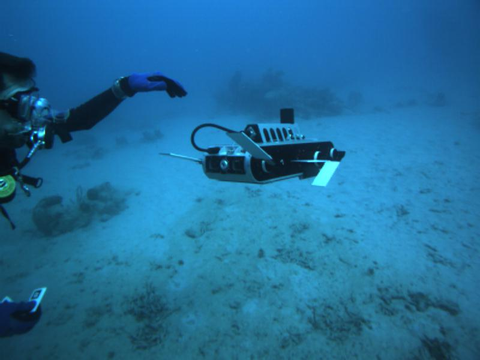
\includegraphics[width=0.21\textwidth]{figures/intermediate/robot_input.png}   & 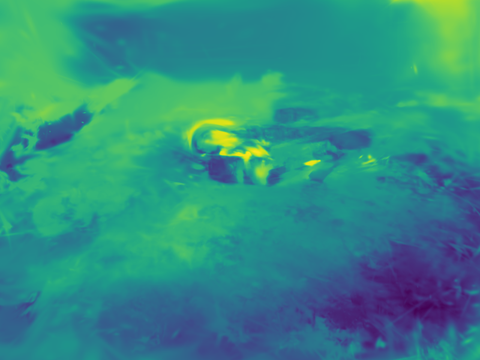
\includegraphics[width=0.21\textwidth]{figures/intermediate/robot_depth.png}   & 
\includegraphics[width=0.21\textwidth]{figures/intermediate/robot_atten.png}   & 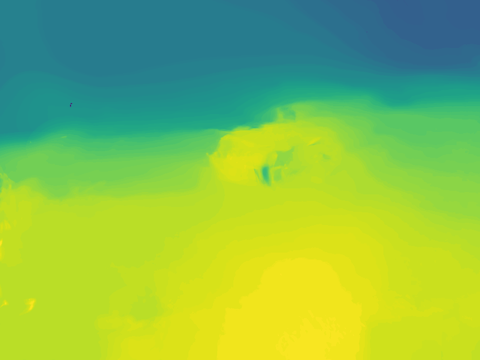
\includegraphics[width=0.21\textwidth]{figures/intermediate/robot_bs.png}   \\
    \rotatebox{90}{Coral}   & 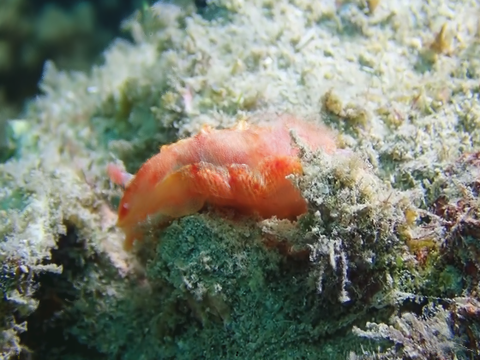
\includegraphics[width=0.21\textwidth]{figures/intermediate/coral_input.png}   & 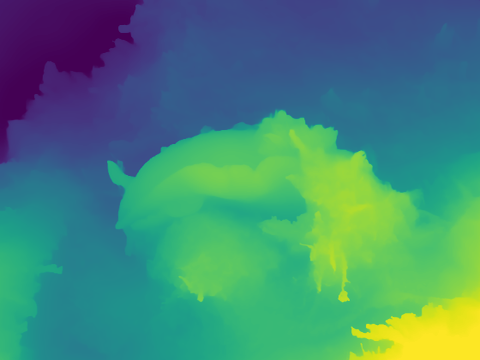
\includegraphics[width=0.21\textwidth]{figures/intermediate/coral_depth.png}   & 
\includegraphics[width=0.21\textwidth]{figures/intermediate/coral_atten.png}   & 
\includegraphics[width=0.21\textwidth]{figures/intermediate/coral_bs.png}   \\
    \rotatebox{90}{Fish}    & 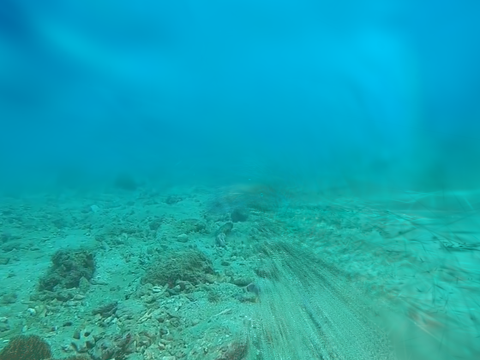
\includegraphics[width=0.21\textwidth]{figures/intermediate/fish_input.png}    & 
\includegraphics[width=0.21\textwidth]{figures/intermediate/fish_depth.png}    & 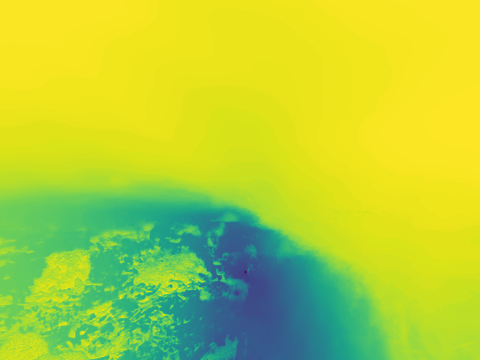
\includegraphics[width=0.21\textwidth]{figures/intermediate/fish_atten.png}    & 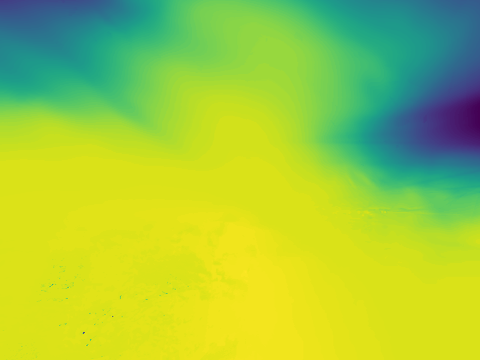
\includegraphics[width=0.21\textwidth]{figures/intermediate/fish_bs.png}    \\
    \rotatebox{90}{Streaks} & 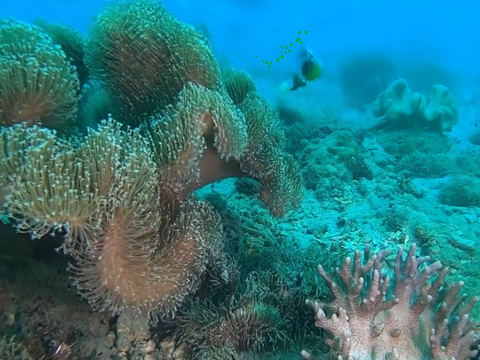
\includegraphics[width=0.21\textwidth]{figures/intermediate/streaks_input.png} & 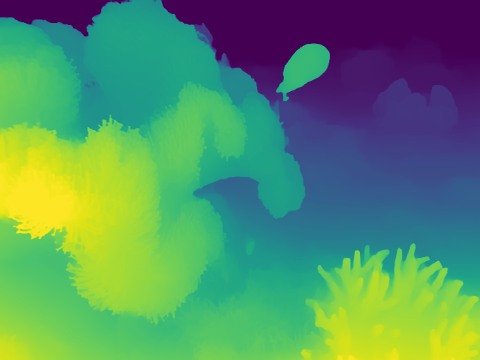
\includegraphics[width=0.21\textwidth]{figures/intermediate/streaks_depth.png} & 
\includegraphics[width=0.21\textwidth]{figures/intermediate/streaks_atten.png} & 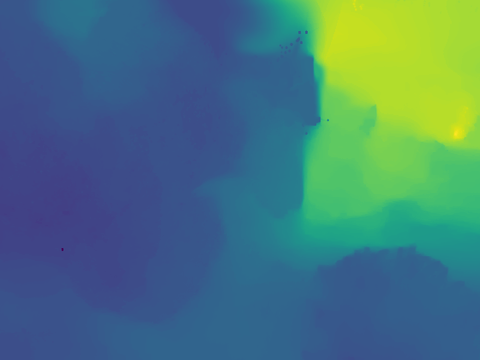
\includegraphics[width=0.21\textwidth]{figures/intermediate/streaks_bs.png} \\
  \end{tabular}
  \caption{四个动态水下场景的中间产物可视化。从左至右依次为：原始输入图像、估计深度图$\mathbf{Z}$、衰减图 $\mathbf{A}(\mathbf{Z})$（$A_c(Z)=\exp(-\beta_c^D Z)$ 逐元素）与后向散射 $\mathbf{B}(\mathbf{Z})$（$B_c(Z)=B_c^\infty(1-\exp(-\beta_c^B Z))$ 逐元素）。深度图采用热力图显示，仅表示相对远近关系。}
  \label{fig:intermediate}
\end{figure}

从图\ref{fig:intermediate}可以看出，估计深度图在主体物体轮廓和背景层次上保持了较连续的相对远近关系，说明单目深度监督对几何结构具有约束作用。衰减图$\mathbf{A}(\mathbf{Z})$在远景区域整体更低，后向散射图$\mathbf{B}(\mathbf{Z})$在较远区域通常更高，这与水下成像模型中"直接透射随距离衰减、后向散射随距离累积"的趋势一致。由于本文没有真实水体光学参数作为监督，上述中间产物只能作为物理趋势和可解释性的辅助证据，不能单独视为参数估计精度的严格验证。

\section{消融实验}

为系统评估本文方法中各核心组件的实际贡献，并揭示水下物理模型在不同场景特性下的适用边界，本文设计了组件解耦实验方案。本节将各场景置于相同硬件预算与相同初始化条件下，仅切换模型组件配置，从而准确隔离各模块的边际贡献。

\subsection{消融实验设计}

本文将完整模型分解为以下四种配置：

\begin{itemize}
  \item \textbf{（a）}仅保留时空高斯溅射主干，关闭水下物理模型与单目深度监督。
  \item \textbf{（b）}启用 SeaThru 物理模型（后向散射$\mathbf{B}(\mathbf{Z})$与衰减$\mathbf{A}(\mathbf{Z})$双子网络），但不引入深度监督。
  \item \textbf{（c）}仅启用基于 Depth Anything V2 的逆深度监督。
  \item \textbf{（d）}同时启用 SeaThru 物理模型与深度监督，即本文完整方法。
\end{itemize}

四种配置在 Robot、Fish、Coral、Streaks 四个动态场景上运行。

\subsection{定量结果}

表\ref{tab:ablation_psnr}给出了四种配置在四个场景上的 PSNR 定量结果。

\begin{table}[htbp]
  \centering
  \tablecaption{消融实验（PSNR / dB）}
  \label{tab:ablation_psnr}
  \begin{tabular}{lcccc}
    \hline
    \textbf{场景} & \textbf{a} & \textbf{b} & \textbf{c} & \textbf{d} \\
    \hline
    Robot   & 29.49               & 29.40                 & 29.24               & \textbf{29.71} \\
    Fish    & \textbf{29.09}      & 27.92     & 28.54               & 28.52 \\
    Coral   & 31.14               & 32.02     & \textbf{33.44}      & 33.29 \\
    Streaks & 28.81               & 30.50                 & \textbf{30.78}      & 30.65 \\
    \hline
  \end{tabular}
\end{table}

表\ref{tab:ablation_ssim_lpips}进一步给出 SSIM 与 LPIPS 指标，便于多维度评估。

\begin{table}[htbp]
  \centering
  \tablecaption{消融实验补充指标（SSIM$\uparrow$ / LPIPS$\downarrow$)}
  \label{tab:ablation_ssim_lpips}
  \begin{tabular}{lcccc}
    \hline
    \textbf{场景} & \textbf{a} & \textbf{b} & \textbf{c} & \textbf{d} \\
    \hline
    Robot   & 0.931 / \textbf{0.066} & 0.934 / 0.163 & 0.932 / 0.165 & \textbf{0.939} / 0.159 \\
    Fish    & 0.821 / 0.139 & 0.816 / 0.155 & 0.822 / 0.137 & \textbf{0.822 / 0.137} \\
    Coral   & 0.927 / 0.061 & 0.956 / 0.076 & \textbf{0.966} / 0.049 & 0.964 / \textbf{0.049} \\
    Streaks & 0.862 / 0.096 & 0.929 / 0.075 & \textbf{0.939} / 0.061 & 0.935 / \textbf{0.061} \\
    \hline
  \end{tabular}
\end{table}

由表\ref{tab:ablation_psnr}与表\ref{tab:ablation_ssim_lpips}可观察到，完整模型并非在所有场景上均为最优。完整模型在Robot上以29.71 dB取得最优PSNR；在Fish场景上，基础4DGS配置（29.09 dB）以约0.57 dB领先完整模型（28.52 dB）；在Coral与Streaks场景上，完整模型（33.29、30.65 dB）相较基础4DGS配置（31.14、28.81 dB）分别提升+2.15 dB和+1.84 dB。以下分析均以两张消融表的数值差异和图\ref{fig:ablation_qualitative}的可视化结果为依据，不额外假设未观测的水体参数。

\subsection{Robot 场景}

Robot场景中，完整模型的PSNR为29.71 dB，高于基础4DGS配置的29.49 dB，也高于仅引入水下物理模型配置的29.40 dB和仅引入深度监督配置的29.24 dB。该结果说明，在机械臂运动相对规则的情况下，单独加入一个组件并不一定带来稳定增益，但水下物理模型和深度监督共同使用时能够互相约束：深度监督减少几何漂移，水下物理模型则对颜色衰减和后向散射进行补偿。SSIM从基础配置的0.931提升至完整模型的0.939，也支持完整模型在结构保持上更稳定。

\subsection{Streaks 场景}

Streaks场景中，基础4DGS配置的PSNR为28.81 dB，仅引入水下物理模型后提升至30.50 dB，仅引入深度监督后进一步提升至30.78 dB，完整模型为30.65 dB。由此可见，两类组件均能改善该场景，但深度监督带来的增益更大；完整模型略低于仅深度监督配置0.13 dB，说明水下物理模型在该场景中并没有提供额外的正向叠加。

这一现象与Streaks场景的外观特征相符：该场景主要挑战是随时间变化的光纹和局部亮度条纹，而式\eqref{eq:uwmodel}中的后向散射项主要描述随深度累积的介质颜色贡献。若动态光纹被水下物理模型部分吸收为介质项，可能会削弱形变网络和深度监督对真实时变外观的表达。因此，在Streaks场景中，本文更倾向于将性能提升归因于深度监督带来的几何稳定性，而不是简单归因于完整水下物理模型。

\subsection{Coral 场景}

Coral场景中，基础4DGS配置的PSNR为31.14 dB，仅引入水下物理模型提升至32.02 dB，仅引入深度监督提升至33.44 dB，完整模型为33.29 dB。该结果说明，Coral场景对深度监督较为敏感，几何约束是主要增益来源；水下物理模型也带来一定提升，但与深度监督叠加后没有超过仅深度监督配置。考虑到Coral场景中珊瑚枝条细碎且存在缓慢摆动，单目深度先验可以直接约束枝条与背景之间的层次关系，因此对PSNR和SSIM的提升更明显。

\subsection{Fish 场景}

Fish场景中，基础4DGS配置取得29.09 dB，高于仅水下物理模型配置的27.92 dB、仅深度监督配置的28.54 dB和完整模型的28.52 dB。该结果表明，对于鱼体快速游动且遮挡变化明显的场景，额外物理分解和深度先验都可能受到动态区域不一致监督的影响。本文方法在该场景的LPIPS与仅深度监督配置接近，但PSNR没有超过基础4DGS，说明当前联合优化策略对高速非刚性运动仍不够稳健。

\subsection{消融实验综合分析}

综合四个场景可以看出，水下物理模型和深度监督的收益依赖场景条件，并不存在对所有场景都最优的固定配置。根据消融结果，本文将影响因素概括为三个维度：水体退化强度、外观变化是否主要由深度相关介质效应造成、运动复杂度。该划分仅用于解释实验现象：当运动较稳定且水体退化明显时，完整模型更容易获得收益；当高速非刚性运动或时变光纹占主导时，额外物理参数可能引入优化负担，需要更谨慎地设置损失权重和训练阶段。

图\ref{fig:ablation_qualitative}以Robot场景为例，给出四种消融配置的渲染效果以及对应的深度图。图中(a)--(d)四列与表\ref{tab:ablation_psnr}中的四种配置一一对应，用于辅助观察不同组件对场景外观与几何重建的影响。

% 红框工具宏：在图像归一化坐标 (0.30,0.20)-(0.70,0.65) 区域绘制红色矩形以突出差异。
% (0,0)=左下，(1,1)=右上；如需调整位置可直接修改本宏定义中的坐标。
\providecommand{\hlimg}[2]{%
  \begin{tikzpicture}[inner sep=0]
    \node[anchor=south west] (im) {\includegraphics[width=#1]{#2}};
    \begin{scope}[x={(im.south east)},y={(im.north west)}]
      \draw[red,very thick] (0.30,0.20) rectangle (0.70,0.65);
    \end{scope}
  \end{tikzpicture}%
}

\begin{figure}[htbp]
  \centering
  \setlength{\tabcolsep}{1pt}
  \renewcommand{\arraystretch}{0.6}
  \begin{tabular}{@{}>{\centering\arraybackslash}m{1.2em}@{\hspace{2pt}}*{4}{>{\centering\arraybackslash}m{0.21\textwidth}}@{}}
     &  &  &  &  \\
    \rotatebox{90}{渲染} & \hlimg{0.21\textwidth}{figures/ablation/a_plain_render.png}  & \hlimg{0.21\textwidth}{figures/ablation/b_seathru_render.png}  & \hlimg{0.21\textwidth}{figures/ablation/c_depthonly_render.png}  & \hlimg{0.21\textwidth}{figures/ablation/d_full_render.png}  \\
    \rotatebox{90}{深度} & \hlimg{0.21\textwidth}{figures/ablation/a_plain_depth.png}   & \hlimg{0.21\textwidth}{figures/ablation/b_seathru_depth.png}   & \hlimg{0.21\textwidth}{figures/ablation/c_depthonly_depth.png}   & \hlimg{0.21\textwidth}{figures/ablation/d_full_depth.png}   \\
     & (a) & (b) & (c) & (d) \\
  \end{tabular}
  \caption{消融实验定性结果（Robot场景），红框标出各配置间差异最显著的区域。各列对应不同消融配置：(a)仅保留时空高斯溅射主干；(b)在(a)之上启用SeaThru水下物理模型；(c)在(a)之上仅启用基于Depth Anything V2的逆深度监督；(d)同时启用SeaThru物理模型与深度监督，即本文完整方法。上行为渲染结果，下行为对应深度图，下标(a)--(d)按老师建议置于图下。}
  \label{fig:ablation_qualitative}
\end{figure}

\subsection{分阶段训练策略消融实验}

为验证实验流程中分阶段训练设计的作用，本节围绕完整流程中的三个关键环节进行消融：粗训练阶段、SeaThru物理分支预热阶段，以及fine阶段初始的高斯参数短暂冻结。完整流程首先在0--3000次迭代中仅优化4D高斯表示，不启用SeaThru物理模型；进入fine阶段后，用学习到的背景初始化后向散射无穷远项，并短暂冻结非颜色高斯参数；随后进行1000次BackscatterNet/AttenuateNet预热、2000次高斯颜色调整，最后进入高斯表示与水下物理分支的间歇联合优化。

参考实验流程消融记录，本文在Robot、Fish、Coral、Streaks四个动态场景上比较不同训练配置。由于部分失败配置的后处理渲染结果存在空白帧或NaN高斯导致的渲染失败，本节不再使用这些不可靠图像作为定性对比，主要依据训练日志、测试集PSNR和稳定性记录进行分析。

\subsubsection{实验配置}

表~\ref{tab:ablation_training_config}给出了本节比较的训练流程配置。0 warmup用于检验物理分支预热是否必要；200 iter与500 iter warmup用于观察最短稳定预热长度；跳过coarse阶段用于验证几何初始化的重要性；取消短暂冻结则用于区分freeze机制与预热机制的相对贡献。

\begin{table}[htbp]
  \centering
  \tablecaption{训练流程消融配置}
  \label{tab:ablation_training_config}
  \small
  \begin{tabular}{p{0.24\textwidth}p{0.22\textwidth}p{0.40\textwidth}}
    \hline
    \textbf{配置} & \textbf{被移除或缩短的环节} & \textbf{实验目的} \\
    \hline
    0 warmup & 移除coarse、预热和freeze & 检验从第1次迭代同时优化高斯、BS/AT与深度监督是否稳定 \\
    200 iter warmup & 移除coarse，仅保留极短预热 & 检验少量预热能否避免立即崩溃 \\
    500 iter warmup & 将coarse与SeaThru开启提前到500次迭代附近 & 检验较短预热在不同场景上的稳定性边界 \\
    跳过coarse，保留完整预热 & 移除0--3000次高斯几何初始化 & 单独检验coarse阶段对几何与后续物理优化的影响 \\
    取消短暂freeze & 保留默认coarse与预热，仅取消fine初始冻结 & 检验freeze是否为主要稳定来源 \\
    \hline
  \end{tabular}
\end{table}

\subsubsection{定量结果}

表~\ref{tab:ablation_training_psnr}汇总了各配置的代表性测试集PSNR。对于训练能够完成但后处理渲染失败的配置，表中采用训练过程中保存的测试集评估值；对于发生CUDA错误或后处理失败的配置，在稳定性列中单独说明。

\begin{table}[htbp]
  \centering
  \tablecaption{训练流程消融实验结果（PSNR / dB）}
  \label{tab:ablation_training_psnr}
  \small
  \begin{tabular}{p{0.25\textwidth}ccccp{0.19\textwidth}}
    \hline
    \textbf{训练配置} & \textbf{Robot} & \textbf{Fish} & \textbf{Coral} & \textbf{Streaks} & \textbf{稳定性摘要} \\
    \hline
    0 warmup & 14.62 & 13.30 & 10.75 & 13.57 & 全部场景持续NaN或停滞 \\
    200 iter warmup，无coarse & 25.98 & 26.68 & 13.82 & 20.58 & 可避免部分崩溃，但Fish后处理渲染失败，Coral质量较低 \\
    500 iter warmup & 26.35 & 26.63 & 19.24 & 19.75 & 训练稳定，但复杂场景质量仍受限 \\
    跳过coarse，保留完整预热 & 28.69 & 18.71 & 6.82 & 10.96 & Robot可训练，其余场景明显退化或崩溃 \\
    取消短暂freeze & 28.11 & 26.77 & 23.57 & 20.21 & 整体稳定，说明freeze不是主要瓶颈 \\
    \hline
  \end{tabular}
\end{table}

从表~\ref{tab:ablation_training_psnr}可以看出，完全取消预热会使四个场景的PSNR均跌至10--15 dB区间，训练日志中伴随长时间NaN梯度警告或训练停滞。200次迭代的极短预热能够降低立即崩溃的概率，例如Fish训练过程中的测试PSNR可恢复到26 dB以上，但后处理渲染仍可能因为NaN高斯失败；Coral场景PSNR仅为13.82 dB，说明极短预热只能缓解数值崩溃，并不能保证复杂场景的几何与物理分解质量。500次迭代预热在四个场景上均能稳定完成训练，但Coral与Streaks仍明显低于理想结果，表明“稳定训练”和“充分重建质量”并不等价。

跳过coarse阶段的结果进一步说明，粗训练提供的几何初始化是复杂场景收敛的前提。Robot场景规模较小、运动和结构相对简单，即使移除coarse阶段仍可保持28 dB以上的PSNR；但Fish、Coral和Streaks在相同设置下分别降至18.71 dB、6.82 dB和10.96 dB，其中Streaks在fine初期曾达到较高PSNR，随后在水下物理分支介入后快速崩溃。这说明coarse阶段并非只提升初始指标，而是在后续SeaThru物理建模中提供稳定几何基础。

\subsubsection{稳定性分析}

表~\ref{tab:ablation_training_stability}给出了训练稳定性的日志摘要。这里不再简单统计最终是否完成训练，而是区分“训练完成但后处理失败”“训练中发生CUDA错误”和“训练完成但质量崩溃”等情况。

\begin{table}[htbp]
  \centering
  \tablecaption{训练流程消融实验稳定性摘要}
  \label{tab:ablation_training_stability}
  \small
  \begin{tabular}{p{0.24\textwidth}p{0.64\textwidth}}
    \hline
    \textbf{训练配置} & \textbf{日志现象} \\
    \hline
    0 warmup & Robot在1269--19994次迭代持续NaN；Fish、Coral、Streaks也出现长段连续NaN，部分早期实验直接停滞或崩溃。 \\
    200 iter warmup，无coarse & Robot无NaN且训练评估较好；Fish可完成训练但后处理渲染失败；Coral避免CUDA崩溃但PSNR仍低；Streaks可训练但质量有限。 \\
    500 iter warmup & 四个场景训练过程稳定，无明显NaN警告；但复杂场景仍需要更完整的coarse-to-fine流程才能获得更好的最终质量。 \\
    跳过coarse，保留完整预热 & Robot基本稳定；Fish出现大量NaN警告，Coral质量严重退化，Streaks出现由高PSNR到低PSNR的后期崩溃。 \\
    取消短暂freeze & 在默认coarse与预热保留时整体稳定，说明短暂冻结主要起辅助缓冲作用，核心稳定性来自coarse阶段与BS/AT预热。 \\
    \hline
  \end{tabular}
\end{table}

上述结果表明，训练流程中最关键的不是单一的参数开关，而是优化顺序。若一开始同时更新高斯几何、动态变形、BackscatterNet、AttenuateNet以及单目深度监督，多个分支会在几何尚未成形时相互补偿，导致梯度尺度失控。SeaThru预热先让BS/AT在相对固定的渲染输入上学习水下成像残差，coarse阶段则为后续物理分支提供可解释的场景几何。二者结合后，后续的颜色调整与间歇联合优化才有稳定基础。

\subsubsection{实验结论}

训练流程消融实验得到以下结论：
\begin{enumerate}
  \item \textbf{SeaThru预热是稳定训练的必要条件}：0 warmup在所有场景上都导致严重NaN或训练停滞，说明水下物理分支不能与未成形的高斯几何从第1次迭代开始强耦合优化。
  \item \textbf{coarse阶段对复杂动态场景不可替代}：Robot可以在无coarse设置下维持较高PSNR，但Fish、Coral和Streaks明显退化，说明粗训练主要解决复杂场景的几何稳定性，而不是简单增加训练迭代数。
  \item \textbf{短预热只能解决部分数值问题}：200或500次迭代预热可以降低崩溃概率，但不能保证复杂场景的最终质量；完整流程仍需要较充分的coarse-to-fine优化。
  \item \textbf{短暂freeze是辅助机制}：在默认coarse和预热保留时，取消fine初始的短暂freeze仍可稳定训练，说明本文流程的核心贡献来自分阶段优化顺序，而非单独依赖冻结操作。
\end{enumerate}

\subsubsection{对水下物理模型中间产物的影响}

训练流程还会影响深度图、去水图、后向散射图和衰减图等中间产物。图~\ref{fig:intermediate}展示了完整流程下各场景的中间产物。在0 warmup或跳过coarse的配置中，由于几何尚未稳定便开始强制拟合水下物理分支，BackscatterNet和AttenuateNet容易把几何误差解释为介质散射或透射衰减，最终表现为深度不连续、去水颜色异常、后向散射数值失真以及衰减图过暗或过亮。

相比之下，完整流程先建立相对稳定的4D高斯几何，再让BS/AT分支预热并进入间歇联合优化，使物理分支学习到的后向散射与直接透射更符合水下成像趋势。因此，分阶段训练不仅提升最终渲染PSNR，也决定了水下物理分解结果是否具有可解释性。
